% ---------------------------------------
% section : Event Triggering
% ---------------------------------------
\subsection{Trigger}
\label{sec:cmsexperiment:trigger}

% overview
CMS applies a two-tiered trigger system \cite{cms:trigger:Khachatryan:2016bia} to select event of interest. The \acrfull{l1t}, composed of custom hardware processors, uses information from the calorimeters and muon detectors to reduce the event rate from 40 MHz to 100 kHz, within a latency less than 4 $\mu s$. The second level, known as the \acrfull{hlt}, consists of a farm of processors running a version of the full event reconstruction software optimized for fast processing, and reduces the event rate from 100 kHz to 1 kHz and output for data storage.



\subsubsection{Level-1 Trigger}

\begin{figure}[ht]
    \centering
    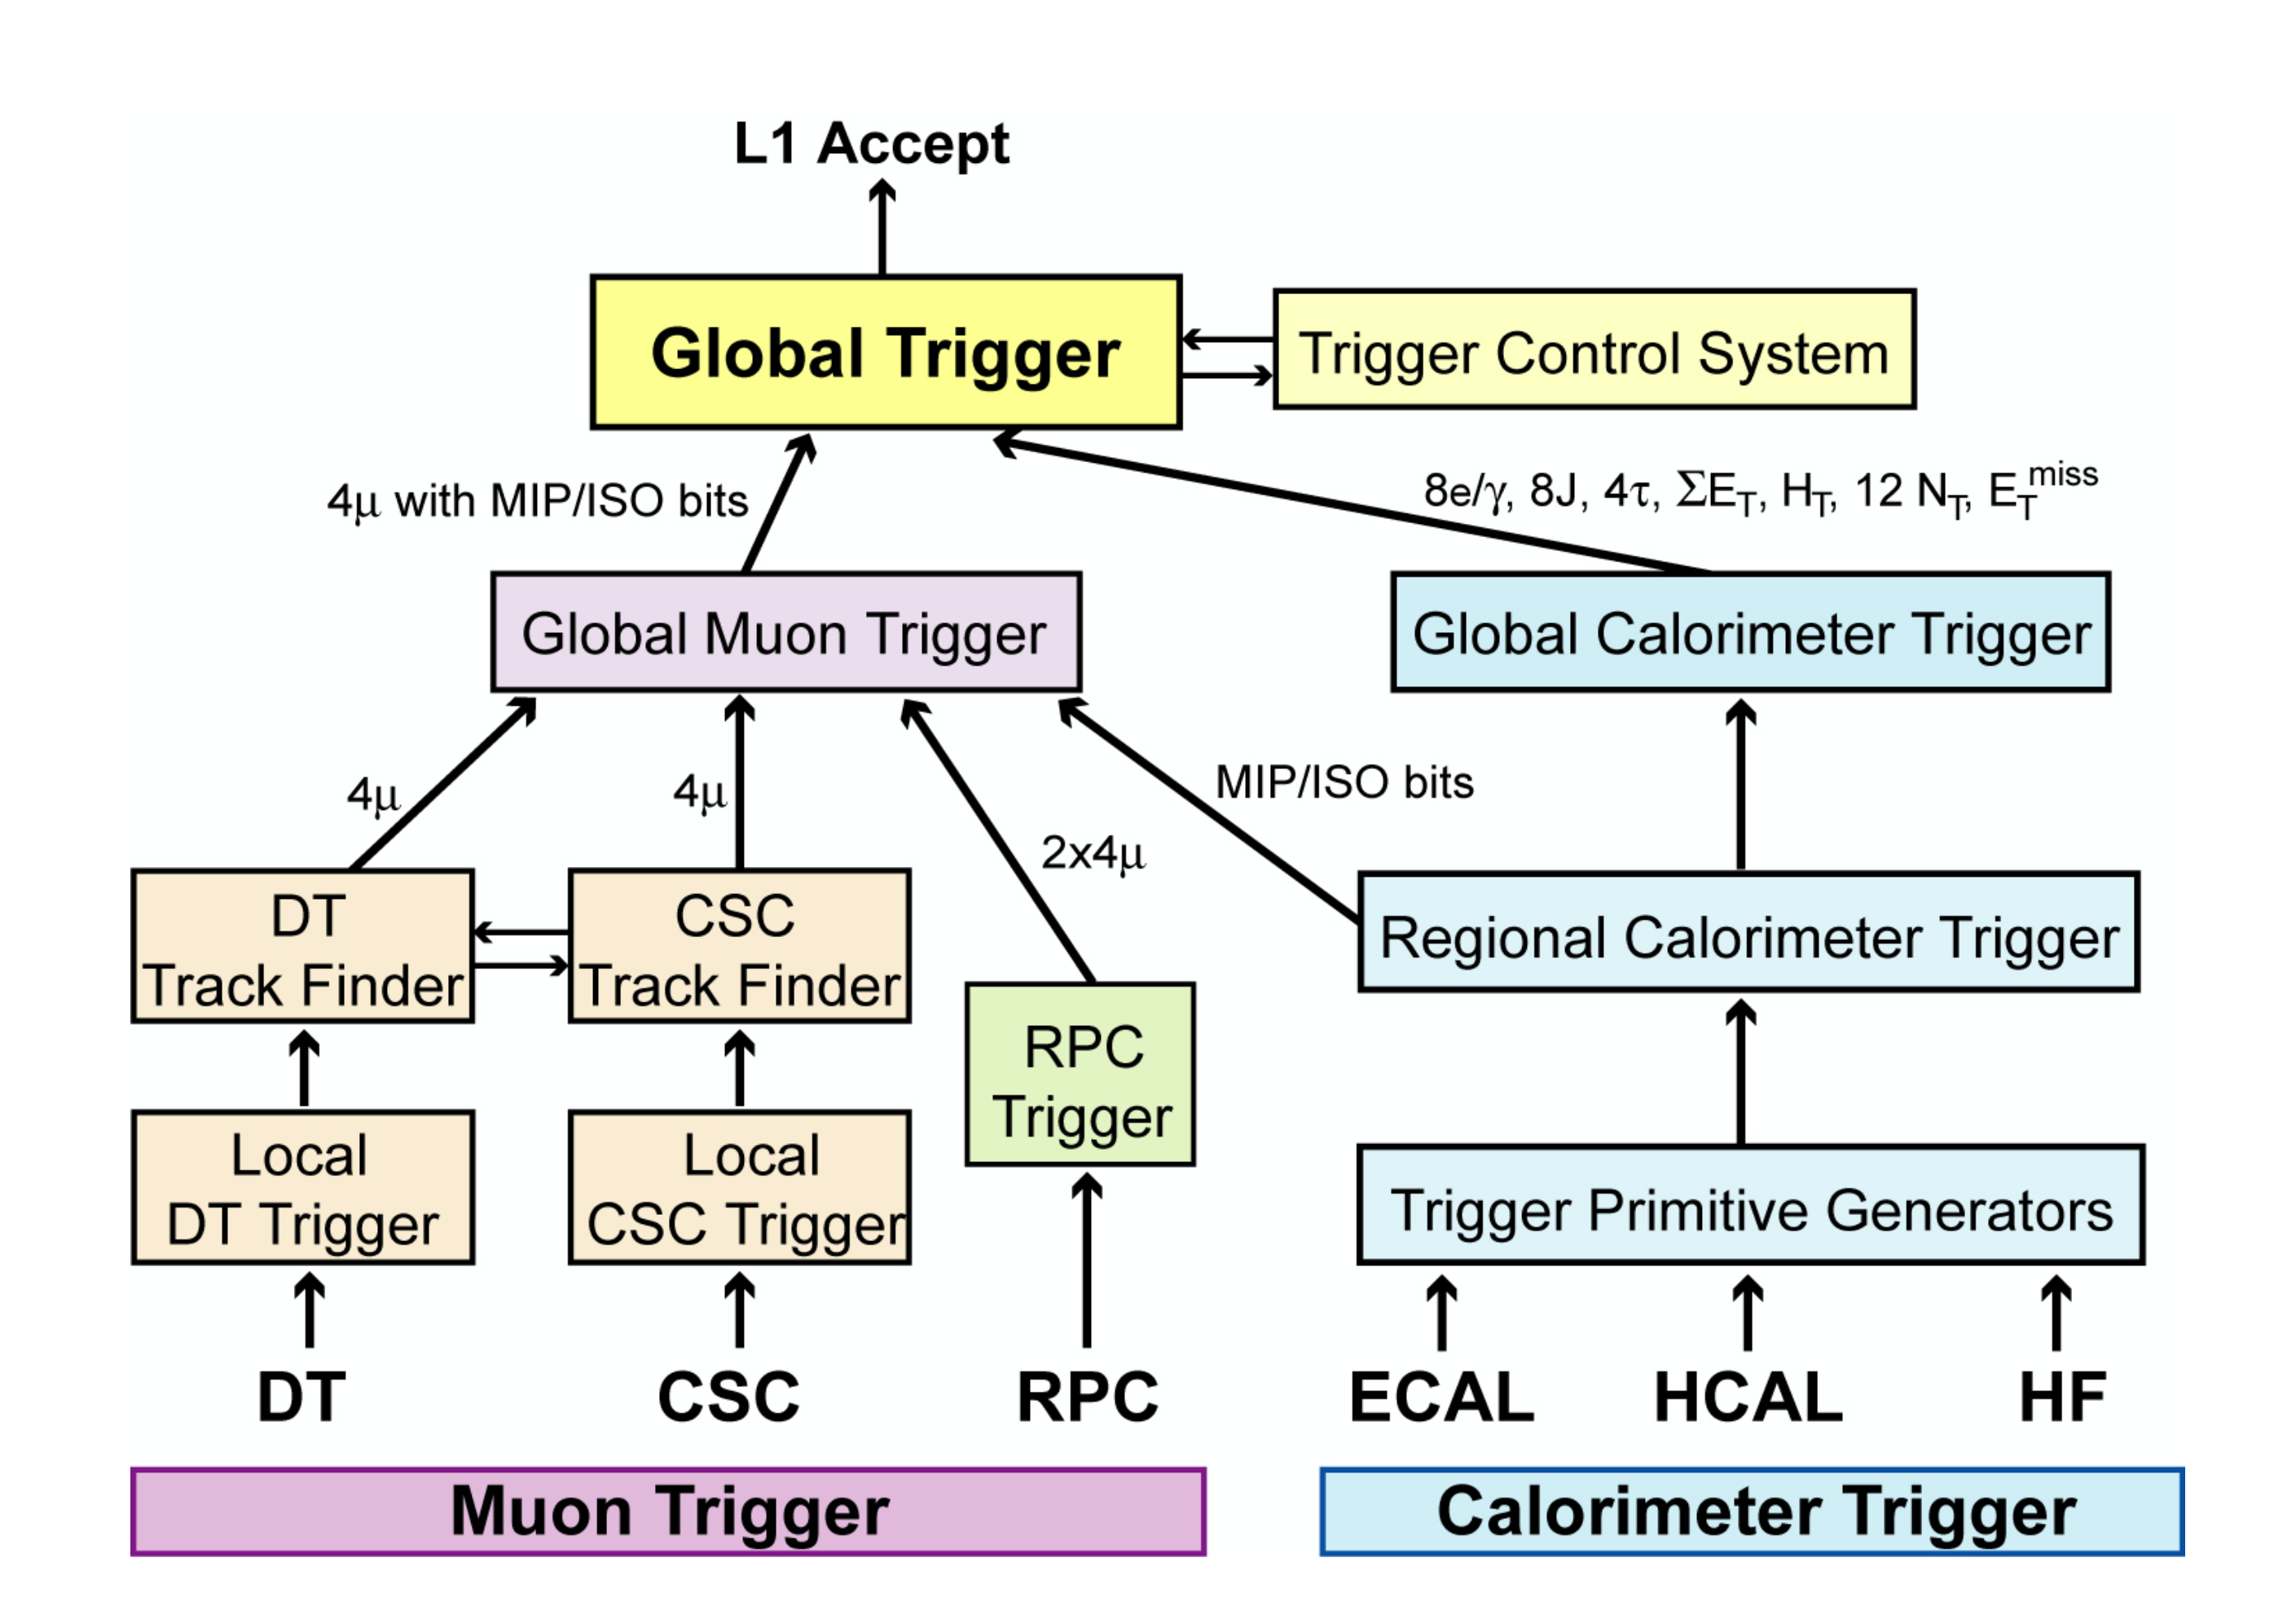
\includegraphics[width=0.8\textwidth]{chapters/CMSExperiment/sectionTrigger/figures/trigger.png}
    \caption{The logic structure of L1T.}
    %  Calorimeters and muon detectors raise local trigger primitives to compute a regional trigger signal. Then \acrfull{gmt} summarizes regional information from DT, SCS and PRC, while \acrfull{gct} concentrates the regional information from ECAL, HCAL and HF. Finally \acrfull{gt} makes the final decision based on the object orientated information from GMT and GCT and transport data in the sub-detectors to the HLT if L1T accept is made. 
    \label{fig:cmsexperiment:trigger:trigger}
\end{figure}

% overview
L1 Trigger is designed to cope with the high collision frequency in the LHC, reducing the event rate from 40 MHz to 100 kHz, keeping only potential events of physics interest. To achieve this, L1 trigger is designed with three component: local, regional and global. The logic structure is shown in Figure~\ref{fig:cmsexperiment:trigger:}. The Local Triggers, also called \acrfull{tpg}, are based on energy deposits in calorimeter trigger towers and track segments or hit patterns in muon chambers. Regional Triggers combine their information and use pattern logic to determine ranked and sorted trigger objects such as electron or muon candidates in limited spatial regions. The \acrfull{gct} and \acrfull{gmt} determine the highest-rank calorimeter and muon objects across the entire experiment and transfer them to the \acrfull{gt}, the top entity of the Level-1 hierarchy. GT takes the decision to reject an event or to accept it for further evaluation by the HLT. The Level-1 Accept decision is communicated to the sub-detectors through the \acrfull{ttc} system. Before decisions arrive to the front-end, the raw data are stored in a FIFO pipelined memories in the front end electronics. Limited by the memory size, only a latency of \SI{3.2}{\us} is allowed between a given bunch crossing and the distribution of the L1T decision to the detector front-end electronics. The L1T electronics is housed partly on the detectors, partly in the underground control room located at a distance of approximately 90 m from the experimental cavern. 


% calo
The \acrfull{tpg} make up the first or local step of the Calorimeter Trigger pipeline. For triggering purposes, the calorimeters are subdivided in trigger towers. The TPGs sum the transverse energies measured in ECAL crystals or HCAL read-out towers to obtain the $E_T$ of the trigger tower and attach the correct bunch crossing number. The TPG electronics is integrated with the calorimeter read-out. The TPGs are transmitted through high-speed serial links to the Regional Calorimeter Trigger, which determines regional candidate electrons/photons, transverse energy sums, $\tau$-veto bits and information relevant for muons in the form of \acrfull{mip} and isolation bits. The Global Calorimeter Trigger determines the highest-rank calorimeter trigger objects across the entire calorimeter system, including 8 $e/\gamma$, 8 jet, 4 $\tau$, $\sum E_T$, $H_T$, 12 $n_j$, met.

% muon
All three muon systems – the DT, the CSC and the RPC – take part in the trigger. The barrel DT chambers provide local trigger information in the form of track segments in the $\phi$-projection and hit patterns in the $\eta$-projection. The endcap CSCs deliver 3-dimensional track segments. All chamber types also identify the bunch crossing from which an event originated. The Regional Muon Trigger consists of the DT and CSC Track Finders, which join segments to complete tracks and assign physical parameters to them. In addition, the RPC trigger chambers, which have excellent timing resolution, deliver their own track candidates based on regional hit patterns. The Global Muon Trigger then combines the information from the three sub-detectors and output 4 leading $\mu$ in the full coverage of muon system, achieving an improved momentum resolution and efficiency compared to the stand-alone systems.

% GT
The GT takes the decision to accept or reject an event at L1 based on trigger objects delivered by the GCT and GMT. The L1T accept decision is communicated to the sub-detectors through the TTC system. Then data corresponding to the triggered bunching crossing is readout from all front-end across the whole detector, as well as L1T objects from GT and send to the HLT.



\subsubsection{High Level Trigger}

The event selection at the HLT is performed in a similar way to that used in the offline processing. For each event, objects such as electrons, muons, and jets are reconstructed and identification criteria are applied in order to select only interested events.

% builder-filter
The HLT hardware consists of a single processor farm composed of commodity computers, the \acrfull{evf}, which runs Scientific Linux. The event filter farm consists of builder-filter units. In the builder units, individual event fragments from the detector are assembled to form complete events. Upon request from a filter unit, the builder unit ships an assembled event to the filter unit. The filter unit in turn unpacks the raw data into detector-specific data structures and performs the event reconstruction and trigger filtering. Associated builder and filter units are located in a single multi-core machine and communicate via shared memory. In total, the EVF executed on approximately 13,000 CPU cores at the end of 2012. On average, the HLT processing time per event is about 90 ms. EVF with 13,000 CPU cores allows a L1T output rate upto 100kHz. With a fixed L1T rate and increasing CPU cores, the allowed time budget for HLT can be expended. The output rate of HLT is limited by the event size and the computing and storage capacity of the offline system.

% filtering and storage
The filtering process uses the full precision of the data from the detector, and the selection is based on offline-quality reconstruction algorithms. It works by computing the a menu of HLT paths, in each of which a predefined process of object reconstruction and event selection is executed. If at least one of the HLT paths get past, the event will be accepted and sent to storage and offline processing. Upon HLT accept decision are made, the events are sent to the storage manager for archival storage. The event data are stored locally on disk and eventually transferred to the CMS Tier-0 computing center for offline processing and permanent storage. Events are grouped into a set of non-exclusive streams according to the HLT decisions.



